\documentclass[12pt, letterpaper]{../assignment}
\usepackage{graphicx}
\usepackage{courier}
\usepackage{minted}
\usepackage{amsmath}
\usepackage{polynom}
\usepackage{commath}
\usepackage{amssymb}
\usepackage{amsfonts} 
\usepackage{color}
\usepackage{cancel}
\usepackage{enumitem}
\usepackage{graphicx}
\usepackage{multirow}
\usepackage{float}
\usepackage{bm}
\usepackage{tikz}
\usetikzlibrary{shapes,arrows}
\usepackage{booktabs}

% Define Theme Colors
\definecolor{light-gray}{rgb}{0.2,0.2,0.2}
\definecolor{header-blue}{rgb}{0,0,0.7}
% \definecolor{header-blue}{rgb}{0.5137,0.8353,0.9176}
\definecolor{header-blue}{rgb}{0,0.8,0.95}
\definecolor{dark-gray}{rgb}{0.1,0.1,0.1}
\pagecolor{dark-gray}
\color{white}

\usemintedstyle{monokai}
\oddsidemargin = 0pt
\exercisesheet{Module 2}{Assignment}
\student{Austin Barrilleaux}
\university{\color{header-blue}Johns Hopkins University}
\school{\color{header-blue}Whiting School of Engineering}
\courselabel{EN 535.612}
\semester{Fall 2024}
\usepackage[backend=bibtex,style=numeric,sorting=none]{biblatex}
\bibliography{reference}

\definecolor{light-gray}{rgb}{0.2,0.2,0.2}
\setminted{bgcolor=light-gray,frame=lines,rulecolor=white}
\setlength{\parindent}{0pt}

\makeatletter
\patchcmd{\minted@colorbg}{\noindent}{\medskip\noindent}{}{}
\apptocmd{\endminted@colorbg}{\par\medskip}{}{}
\makeatother

\begin{document}

\subsection*{Problem 1:}
\subsubsection*{Type I Euler angles are also known as the aircraft Euler angles.
These are comprised of (1) a rotation $\bm{\psi}$ about the fixed $\bm{Z}$-axis, 
resulting in a primed axis system;
(2) a rotation $\bm{\theta}$ about the $\bm{y'}$-axis resulting in a double-primed system;
and (3) a rotation $\bm{\phi}$ about the $\bm{x”}$-axis, resulting in the final $\bm{xyz}$ body-fixed frame.\\
\begin{enumerate}[label=\alph*]
    \item Neatly sketch this sequence of rotations.
    \item Derive the rotation matrix that maps the $\bm{XYZ}$ frame to the body-fixed $\bm{xyz}$ frame.
\end{enumerate}}


The following sketch shows the rotations:
\begin{answer}
\begin{center}
% Holy shit https://www.mathcha.io/editor is awesome!!!
\tikzset{every picture/.style={line width=0.75pt}} %set default line width to 0.75pt        
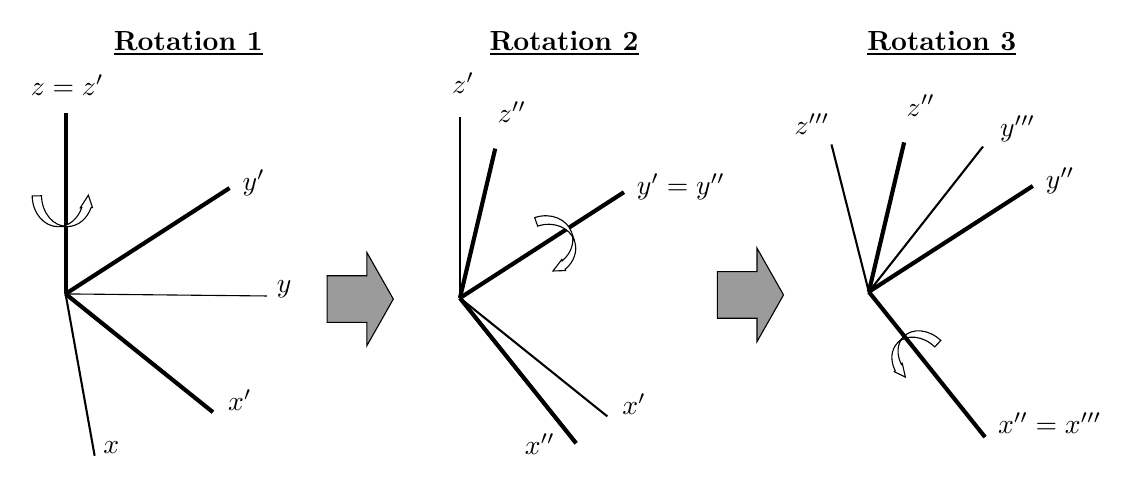
\begin{tikzpicture}[x=0.75pt,y=0.75pt,yscale=-1,xscale=1]
%uncomment if require: \path (0,232); %set diagram left start at 0, and has height of 232
%Straight Lines [id:da5095770286058787] 
\draw [line width=1.5]    (64,138) -- (64,51) ;
%Straight Lines [id:da33738645957574454] 
\draw    (64,138) -- (161,139) ;
%Straight Lines [id:da358096470075816] 
\draw [line width=1.5]    (135,195) -- (64,138) ;
%Straight Lines [id:da7066666899008867] 
\draw [line width=0.75]    (64,138) -- (78,216) ;
%Straight Lines [id:da04175385458180503] 
\draw [line width=1.5]    (64,138) -- (143,87) ;
%Curve Right Arrow [id:dp2536384256344437] 
\draw  [fill={rgb, 255:red, 255; green, 255; blue, 255 }  ,fill opacity=1 ] (65.02,105.56) .. controls (58.16,105.65) and (52.51,99.01) .. (52.4,90.73) -- (47.9,90.79) .. controls (48.01,99.08) and (53.66,105.71) .. (60.52,105.62) ;\draw  [fill={rgb, 255:red, 255; green, 255; blue, 255 }  ,fill opacity=1 ] (60.52,105.62) .. controls (65.61,105.55) and (69.94,101.78) .. (71.78,96.46) -- (71.11,96.47) -- (74.98,90.42) -- (76.94,96.39) -- (76.28,96.4) .. controls (74.44,101.72) and (70.11,105.48) .. (65.02,105.56)(60.52,105.62) -- (65.02,105.56) ;
%Straight Lines [id:da5136698224282734] 
\draw [line width=0.75]    (254,140) -- (254,53) ;
%Straight Lines [id:da48017931107776035] 
\draw [line width=0.75]    (325,197) -- (254,140) ;
%Straight Lines [id:da9660459831351487] 
\draw [line width=1.5]    (254,140) -- (333,89) ;
%Curve Right Arrow [id:dp3545404895300446] 
\draw  [fill={rgb, 255:red, 255; green, 255; blue, 255 }  ,fill opacity=1 ] (309.21,112.49) .. controls (306.97,105.96) and (299.02,102.76) .. (291.44,105.35) -- (290.03,101.24) .. controls (297.61,98.65) and (305.57,101.84) .. (307.8,108.37) ;\draw  [fill={rgb, 255:red, 255; green, 255; blue, 255 }  ,fill opacity=1 ] (307.8,108.37) .. controls (309.46,113.22) and (307.5,118.55) .. (303.28,122.04) -- (303.07,121.43) -- (298.83,126.96) -- (304.9,126.76) -- (304.69,126.15) .. controls (308.91,122.67) and (310.87,117.34) .. (309.21,112.49)(307.8,108.37) -- (309.21,112.49) ;
%Straight Lines [id:da42805597420295083] 
\draw [line width=1.5]    (271,68) -- (254,140) ;
%Straight Lines [id:da5320392133454459] 
\draw [line width=1.5]    (310,210) -- (254,140) ;
%Straight Lines [id:da9906216954206488] 
\draw [line width=1.5]    (451,137) -- (530,86) ;
%Curve Right Arrow [id:dp2193417807817155] 
\draw  [fill={rgb, 255:red, 255; green, 255; blue, 255 }  ,fill opacity=1 ] (464.74,161.71) .. controls (469.04,157.26) and (477.1,158.07) .. (482.74,163.52) -- (485.7,160.46) .. controls (480.07,155.01) and (472.01,154.19) .. (467.7,158.64) ;\draw  [fill={rgb, 255:red, 255; green, 255; blue, 255 }  ,fill opacity=1 ] (467.7,158.64) .. controls (464.5,161.95) and (464.27,167.23) .. (466.67,171.96) -- (467.11,171.5) -- (468.62,178.11) -- (463.27,175.47) -- (463.71,175.02) .. controls (461.31,170.29) and (461.54,165.01) .. (464.74,161.71)(467.7,158.64) -- (464.74,161.71) ;
%Straight Lines [id:da11640722170105056] 
\draw [line width=1.5]    (468,65) -- (451,137) ;
%Straight Lines [id:da7923091571988319] 
\draw [line width=1.5]    (507,207) -- (451,137) ;
%Straight Lines [id:da20015144238386617] 
\draw [line width=0.75]    (451,137) -- (433,66) ;
%Straight Lines [id:da13756437536181032] 
\draw [line width=0.75]    (451,137) -- (506,67) ;
%Right Arrow [id:dp7199747848891722] 
\draw  [fill={rgb, 255:red, 155; green, 155; blue, 155 }  ,fill opacity=1 ] (190,129.25) -- (209.14,129.25) -- (209.14,118) -- (221.9,140.5) -- (209.14,163) -- (209.14,151.75) -- (190,151.75) -- cycle ;
%Right Arrow [id:dp3017426167325514] 
\draw  [fill={rgb, 255:red, 155; green, 155; blue, 155 }  ,fill opacity=1 ] (378,127.25) -- (397.14,127.25) -- (397.14,116) -- (409.9,138.5) -- (397.14,161) -- (397.14,149.75) -- (378,149.75) -- cycle ;
% Text Node
\draw (81,208) node [anchor=north west][inner sep=0.75pt]   [align=left] {$x$};
% Text Node
\draw (141,183) node [anchor=north west][inner sep=0.75pt]   [align=left] {$x'$};
% Text Node
\draw (164.54,130.31) node [anchor=north west][inner sep=0.75pt]   [align=left] {$y$};
% Text Node
\draw (148,77) node [anchor=north west][inner sep=0.75pt]   [align=left] {$y'$};
% Text Node
\draw (46,31) node [anchor=north west][inner sep=0.75pt]   [align=left] {$z = z'$};
% Text Node
\draw (284,204) node [anchor=north west][inner sep=0.75pt]   [align=left] {$x''$};
% Text Node
\draw (331,185) node [anchor=north west][inner sep=0.75pt]   [align=left] {$x'$};
% Text Node
\draw (338,79) node [anchor=north west][inner sep=0.75pt]   [align=left] {$y'=y''$};
% Text Node
\draw (249,30) node [anchor=north west][inner sep=0.75pt]   [align=left] {$z'$};
% Text Node
\draw (271,44) node [anchor=north west][inner sep=0.75pt]   [align=left] {$z''$};
% Text Node
\draw (512,194) node [anchor=north west][inner sep=0.75pt]   [align=left] {$x'' = x'''$};
% Text Node
\draw (513,51) node [anchor=north west][inner sep=0.75pt]   [align=left] {$y'''$};
% Text Node
\draw (535,76) node [anchor=north west][inner sep=0.75pt]   [align=left] {$y''$};
% Text Node
\draw (414,50) node [anchor=north west][inner sep=0.75pt]   [align=left] {$z'''$};
% Text Node
\draw (468,41) node [anchor=north west][inner sep=0.75pt]   [align=left] {$z''$};
% Text Node
\draw (86,10) node [anchor=north west][inner sep=0.75pt]   [align=left] {\underline{\textbf{Rotation 1}}};
% Text Node
\draw (267,10) node [anchor=north west][inner sep=0.75pt]   [align=left] {\underline{\textbf{Rotation 2}}};
% Text Node
\draw (449,10) node [anchor=north west][inner sep=0.75pt]   [align=left] {\underline{\textbf{Rotation 3}}};
\end{tikzpicture}
\end{center}
\end{answer}

This rotation matrix is defined by the following three sequential rotations:

\begin{equation*}
    \begin{aligned}
        R_1 &= \left[\begin{array}{ccc} \cos\left(\psi \right) & \sin\left(\psi \right) & 0\\ -\sin\left(\psi \right) & \cos\left(\psi \right) & 0\\ 0 & 0 & 1 \end{array}\right]\\
        R_2 &= \left[\begin{array}{ccc} \cos\left(\theta \right) & 0 & -\sin\left(\theta \right)\\ 0 & 1 & 0\\ \sin\left(\theta \right) & 0 & \cos\left(\theta \right) \end{array}\right]\\
        R_3 &= \left[\begin{array}{ccc} 1 & 0 & 0\\ 0 & \cos\left(\phi \right) & \sin\left(\phi \right)\\ 0 & -\sin\left(\phi \right) & \cos\left(\phi \right) \end{array}\right]
    \end{aligned}
\end{equation*}

The overall rotation matrix $R$ that maps the $XYZ$ frame to the body-fixed $xyz$ frame is:

$$ R = R_3(\phi)\ R_2(\theta)\ R_1(\psi) $$

Which becomes:

\begin{answer}
$$ \scriptsize R(\phi,\theta,\psi) = \left[\begin{array}{ccc} 
    \cos\left(\psi \right)\cos\left(\theta \right) &
    \cos\left(\theta \right)\sin\left(\psi \right) &
    -\sin\left(\theta \right)\\
    \cos\left(\psi \right)\sin\left(\phi \right)\sin\left(\theta \right)-\cos\left(\phi \right)\sin\left(\psi \right) & 
    \cos\left(\phi \right)\cos\left(\psi \right)+\sin\left(\phi \right)\sin\left(\psi \right)\sin\left(\theta \right) & 
    \cos\left(\theta \right)\sin\left(\phi \right)\\
    \sin\left(\phi \right)\sin\left(\psi \right)+\cos\left(\phi \right)\cos\left(\psi \right)\sin\left(\theta \right) &
    \cos\left(\phi \right)\sin\left(\psi \right)\sin\left(\theta \right)-\cos\left(\psi \right)\sin\left(\phi \right) &
    \cos\left(\phi \right)\cos\left(\theta \right)
\end{array}\right] $$
\end{answer}

This makes sense,
as if I take the transpose of this matrix,
I see the matrix in the space-fixed form that I am used to seeing the transform in the aerospace industry:

$$ \scriptsize R(\phi,\theta,\psi)' = \left[\begin{array}{ccc}
    \cos\left(\psi \right)\,\cos\left(\theta \right) &
    \cos\left(\psi \right)\,\sin\left(\phi \right)\,\sin\left(\theta \right)-\cos\left(\phi \right)\,\sin\left(\psi \right) &
    \sin\left(\phi \right)\,\sin\left(\psi \right)+\cos\left(\phi \right)\,\cos\left(\psi \right)\,\sin\left(\theta \right)\\
    \cos\left(\theta \right)\,\sin\left(\psi \right) &
    \cos\left(\phi \right)\,\cos\left(\psi \right)+\sin\left(\phi \right)\,\sin\left(\psi \right)\,\sin\left(\theta \right) &
    \cos\left(\phi \right)\,\sin\left(\psi \right)\,\sin\left(\theta \right)-\cos\left(\psi \right)\,\sin\left(\phi \right)\\
    -\sin\left(\theta \right) &
    \cos\left(\theta \right)\,\sin\left(\phi \right) &
    \cos\left(\phi \right)\,\cos\left(\theta \right)
\end{array}\right] $$

\subsection*{Problem 2: EXERCISE 3.18}
\subsubsection*{A hydraulic cylinder allows the length of arm $\bm{AB}$ to vary,
and servomotors control the rotation angles $\bm{\theta}$ about the vertical,
$\bm{\beta}$ about pin $\bm{A}$, and $\bm{\gamma}$ about axis $\bm{AB}$,
with $\bm{\gamma = 0}$ corresponding to bar $\bm{BC}$ being situated in the vertical
plane as shown. In the initial position $\bm{L = 250}$ mm, $\bm{\theta = 0}$,
$\bm{\beta = 90^\circ}$,and $\bm{\gamma = 0}$.
In the final position, $\bm{\theta = \beta = 120^\circ}$, $\bm{\gamma = 90^\circ}$,
and $\bm{L = 500}$ mm. Determine the corresponding displacement of end $\bm{C}$.}

\begin{figure}[H]
    \centering
    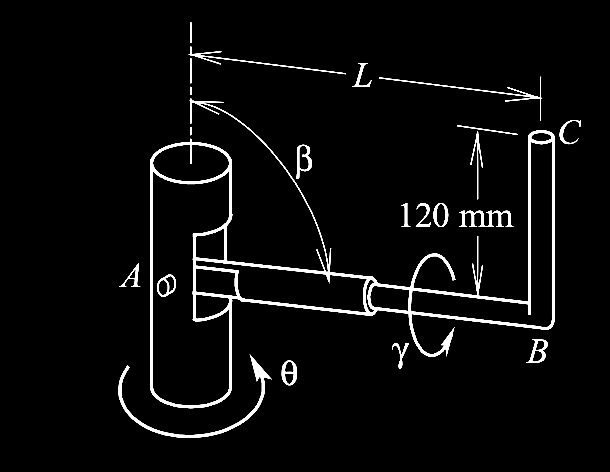
\includegraphics[frame]{images/P_3_18.png}
\end{figure}

We will use the coordinate frame as defined in the following figure:

\begin{figure}[H]
    \centering
    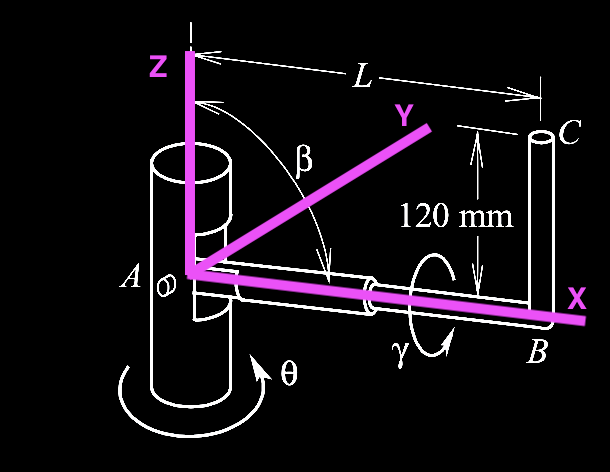
\includegraphics[frame]{images/P_3_18_cf.png}
\end{figure}

Where

\begin{equation*}
    \begin{aligned}
        \left[\begin{array}{c} X' \\ Y' \\ Z' \end{array}\right] =
        R_A \left[\begin{array}{c} X \\ Y \\ Z \end{array}\right]   
    \end{aligned}
\end{equation*}

The rotation about these axes is

\begin{equation*}
    \begin{aligned}
        R_A =  \left[\begin{array}{ccc} \cos\left(\beta-90\right) & 0 & -\sin\left(\beta-90\right)\\ 0 & 1 & 0\\ \sin\left(\beta-90\right) & 0 & \cos\left(\beta-90\right) \end{array}\right]
        \left[\begin{array}{ccc} \cos\left(\theta\right) & \sin\left(\theta\right) & 0\\ -\sin\left(\theta\right) & \cos\left(\theta\right) & 0\\ 0 & 0 & 1 \end{array}\right]
    \end{aligned}
\end{equation*}

This gives

\begin{equation*}
\begin{aligned}
    R_{A_i} &= \left[\begin{array}{ccc} 1 & 0 & 0\\ 0 & 1 & 0\\ 0 & 0 & 1 \end{array}\right]\\
    R_{A_f} &= \left[\begin{array}{ccc} -\frac{\sqrt{3}}{4} & \frac{3}{4} & -\frac{1}{2}\\ -\frac{\sqrt{3}}{2} & -\frac{1}{2} & 0\\ -\frac{1}{4} & \frac{\sqrt{3}}{4} & \frac{\sqrt{3}}{2} \end{array}\right]
\end{aligned}
\end{equation*}

The displacement of point $A$ to $C$ is defined as

$$ \Delta \bar{r}_C = \bar{r}_{{C/A}_f} - \bar{r}_{{C/A}_i}  $$

Where

$$ \bar{r}_{{C/A}_i} = \left[\begin{array}{r} L_i \\-120 \sin(\gamma_i) \\120 \cos(\gamma_i) \end{array}\right]
= \left[\begin{array}{c} 250\\ 0\\ 120 \end{array}\right] \ \text{mm} $$

$$ \bar{r}_{{C/A}_f} = \left[\begin{array}{r} L_f \\-120 \sin(\gamma_f) \\120 \cos(\gamma_f) \end{array}\right]
= \left[\begin{array}{c} 500\\ 120\\ 0 \end{array}\right] \ \text{mm} $$

Therefore

$$ \Delta \bar{r}_C = \bar{r}_{{C/A}_f} - \bar{r}_{{C/A}_i} 
= \left[\begin{array}{r} 250\\ 120\\ -120 \end{array}\right] \ \text{mm} $$

We can compute the displacement of point C in terms of the original axes we defined as

$$ \Delta {\bar{r}_C}' = {R_{A_f}}^T \Delta \bar{r}_C  + \left( {R_{A_f}}^T - {R_{A_i}}^T \right)\bar{r}_{{C/A}_i} = 
\left[\begin{array}{r}  -570.43\\315.00 \\ -370.00 \end{array}\right] \ \text{mm} $$

So the displacement is:

\begin{answer}
$$ \Delta {\bar{r}_C}' =
\left[\begin{array}{r}  -570.43\\315.00 \\ -370.00 \end{array}\right] \ \textbf{mm}, \ \ \
\left|\Delta {\bar{r}_C}'\right| = 749.34 \ \textbf{mm} $$
\end{answer}

% \color{white}
% \hspace*{6em}\inputminted[frame=leftline,fontsize=\footnotesize]{matlab}
% {./matlab/B_2_18.m}
% \color{black} 

% It has the following response, which matches my analytically derived solution:

% \begin{figure}[H]
%     \centering
%     \includegraphics{matlab/B_2_18.png}
%     \caption{Response of the system}
% \end{figure}

\end{document}

